% !TeX spellcheck = en_GB

%%%%%%%
\begin{figure}[t]
	\centering
    % 20/12
		\begin{subfigure}[t]{\textwidth}		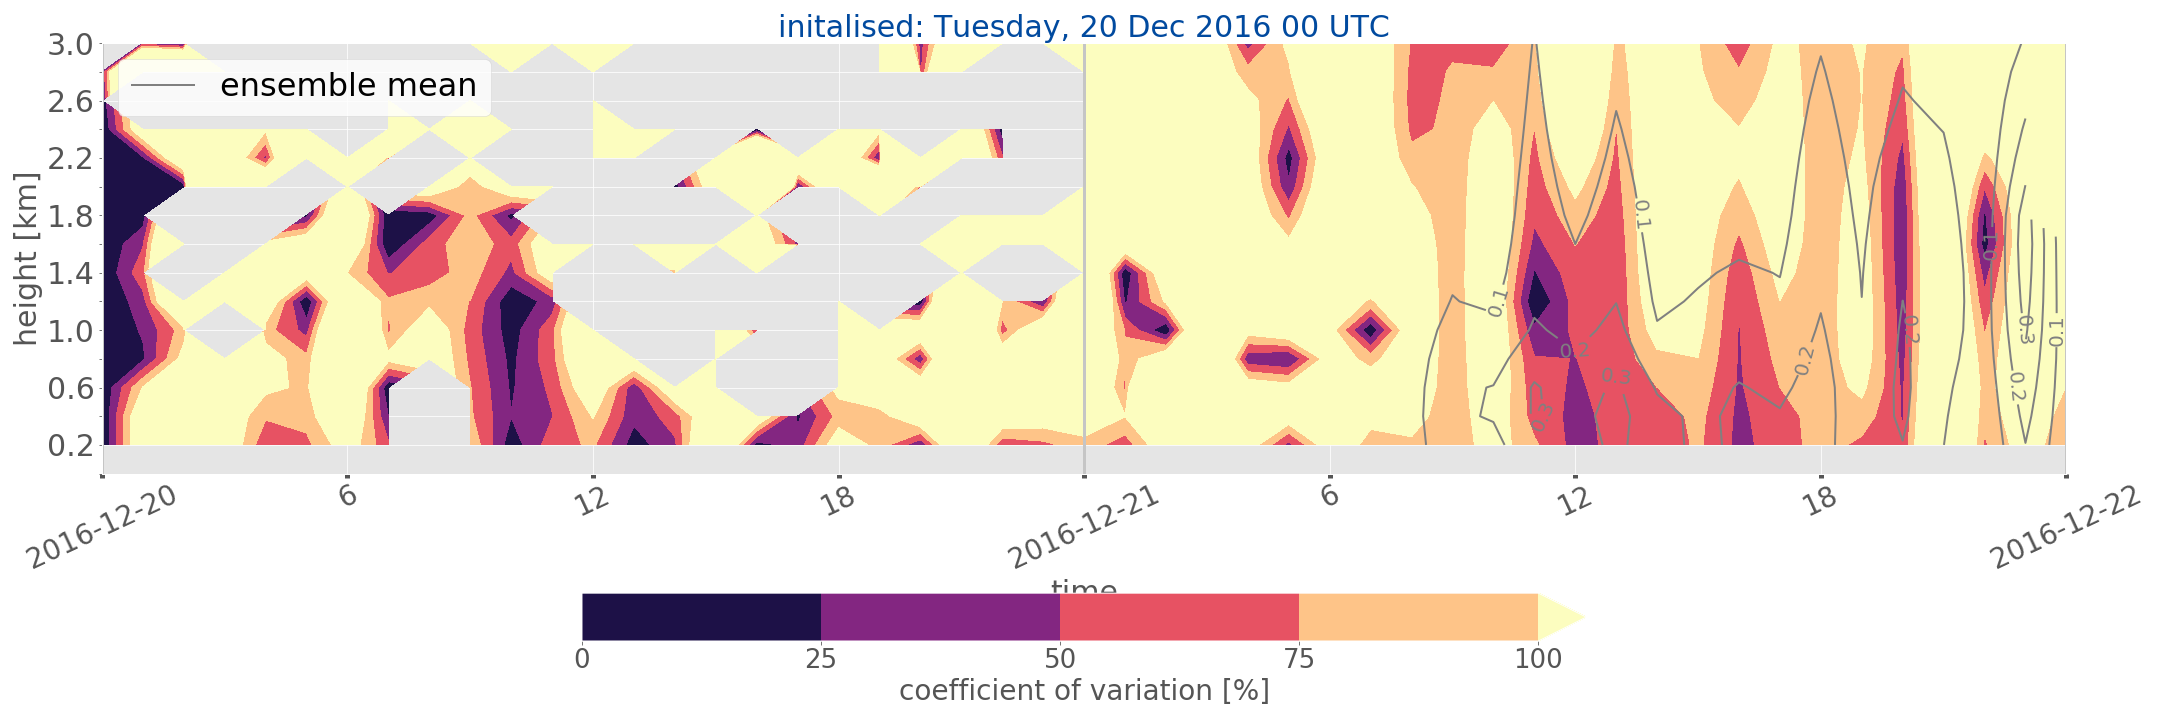
\includegraphics[trim={0.cm 5.3cm 0cm 0cm},clip,width=\textwidth]{./fig_variation/20161220}
			\caption{}\label{fig:ens_vari20}
		\end{subfigure}
%\end{figure}
%\begin{figure}\ContinuedFloat
    % 21/12
		\begin{subfigure}[t]{\textwidth}		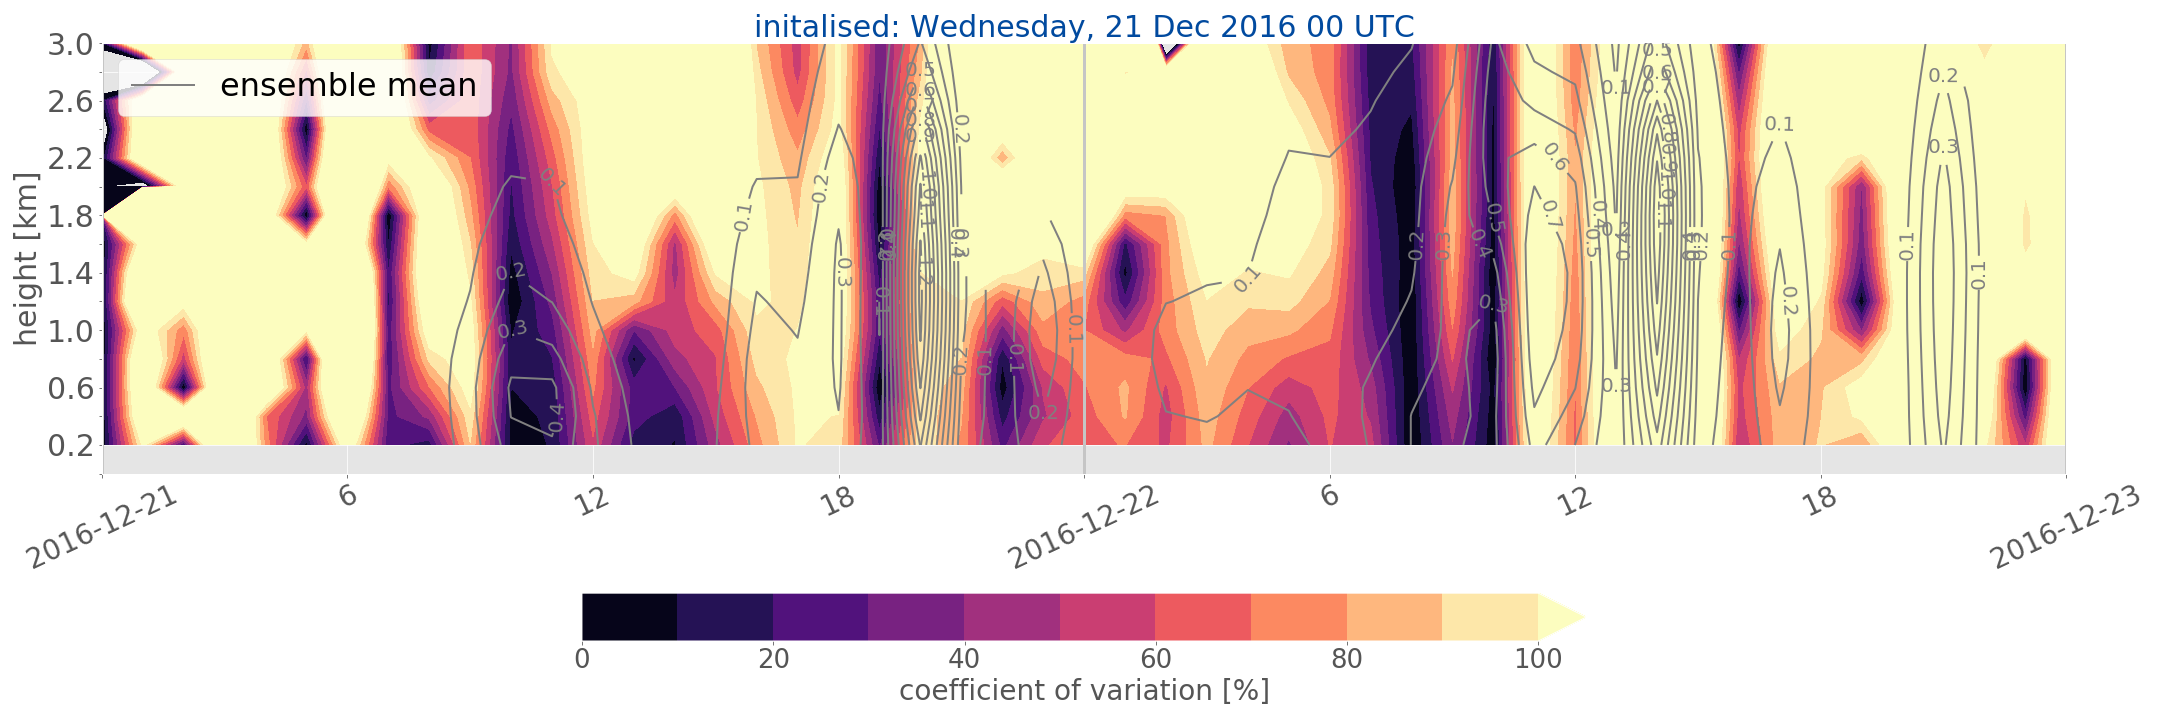
\includegraphics[trim={0.cm 5.3cm 0cm 0cm},clip,width=\textwidth]{./fig_variation/20161221}
			\caption{}\label{fig:ens_vari21}
		\end{subfigure}
       
       % colourbar
     	\begin{subfigure}[t]{\textwidth}		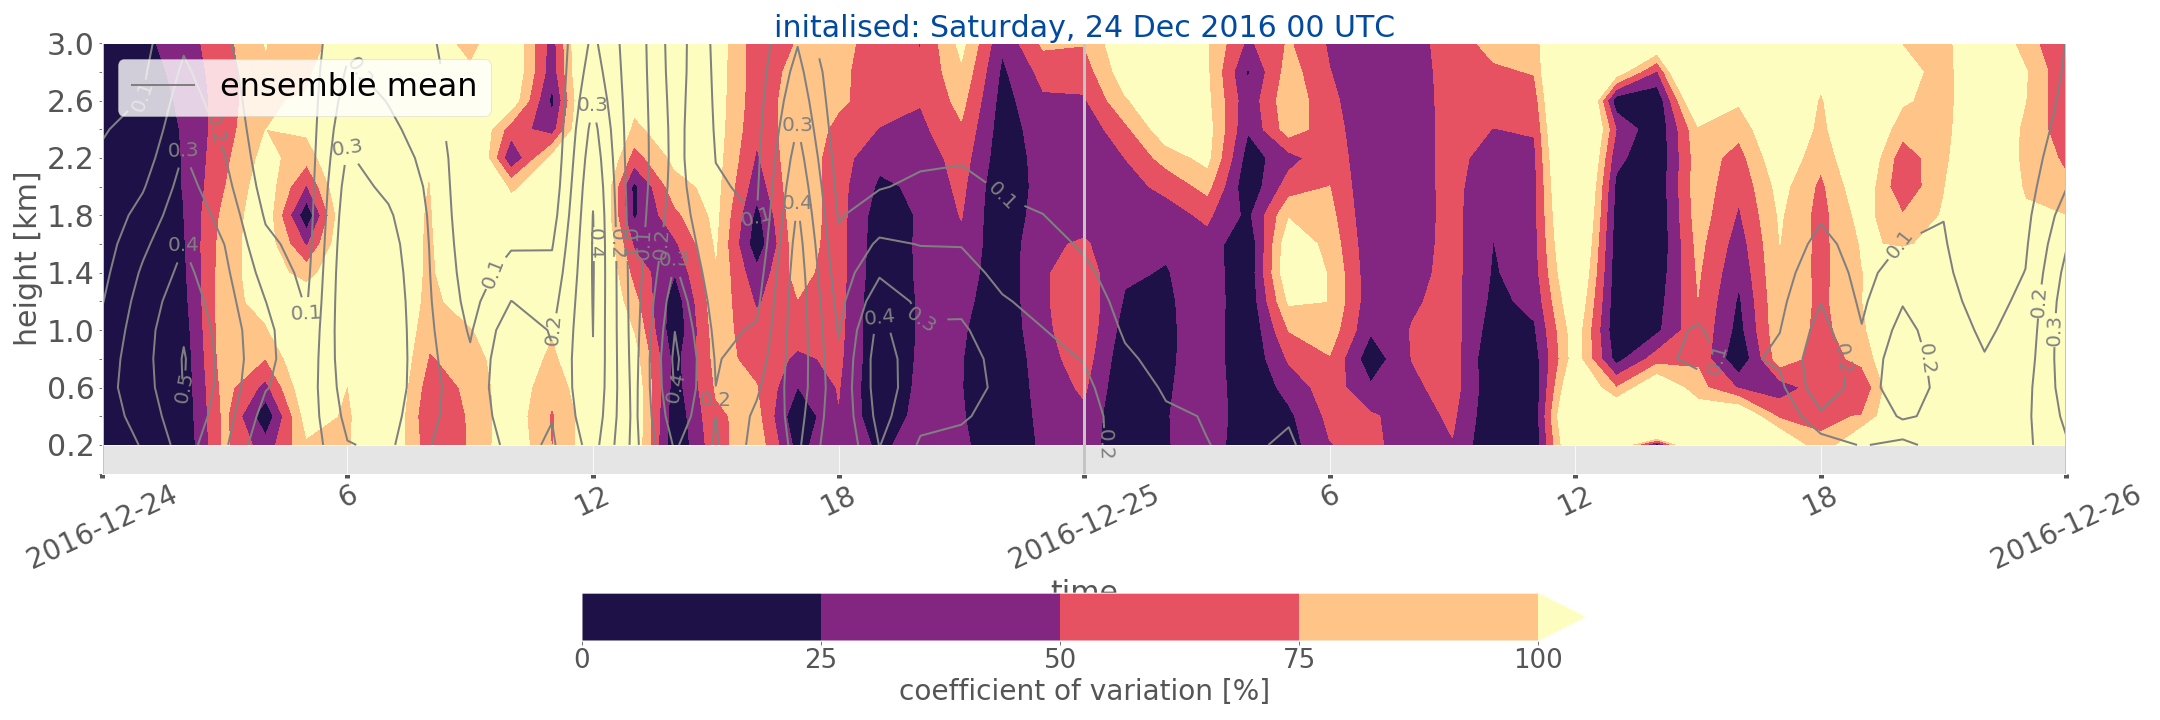
\includegraphics[trim={15.cm 0cm 15cm 21cm},clip,width=\textwidth]{./fig_variation/20161224}
		\end{subfigure}
\end{figure}
\begin{figure}[t]\ContinuedFloat
    % 22/12
		\begin{subfigure}[t]{\textwidth}		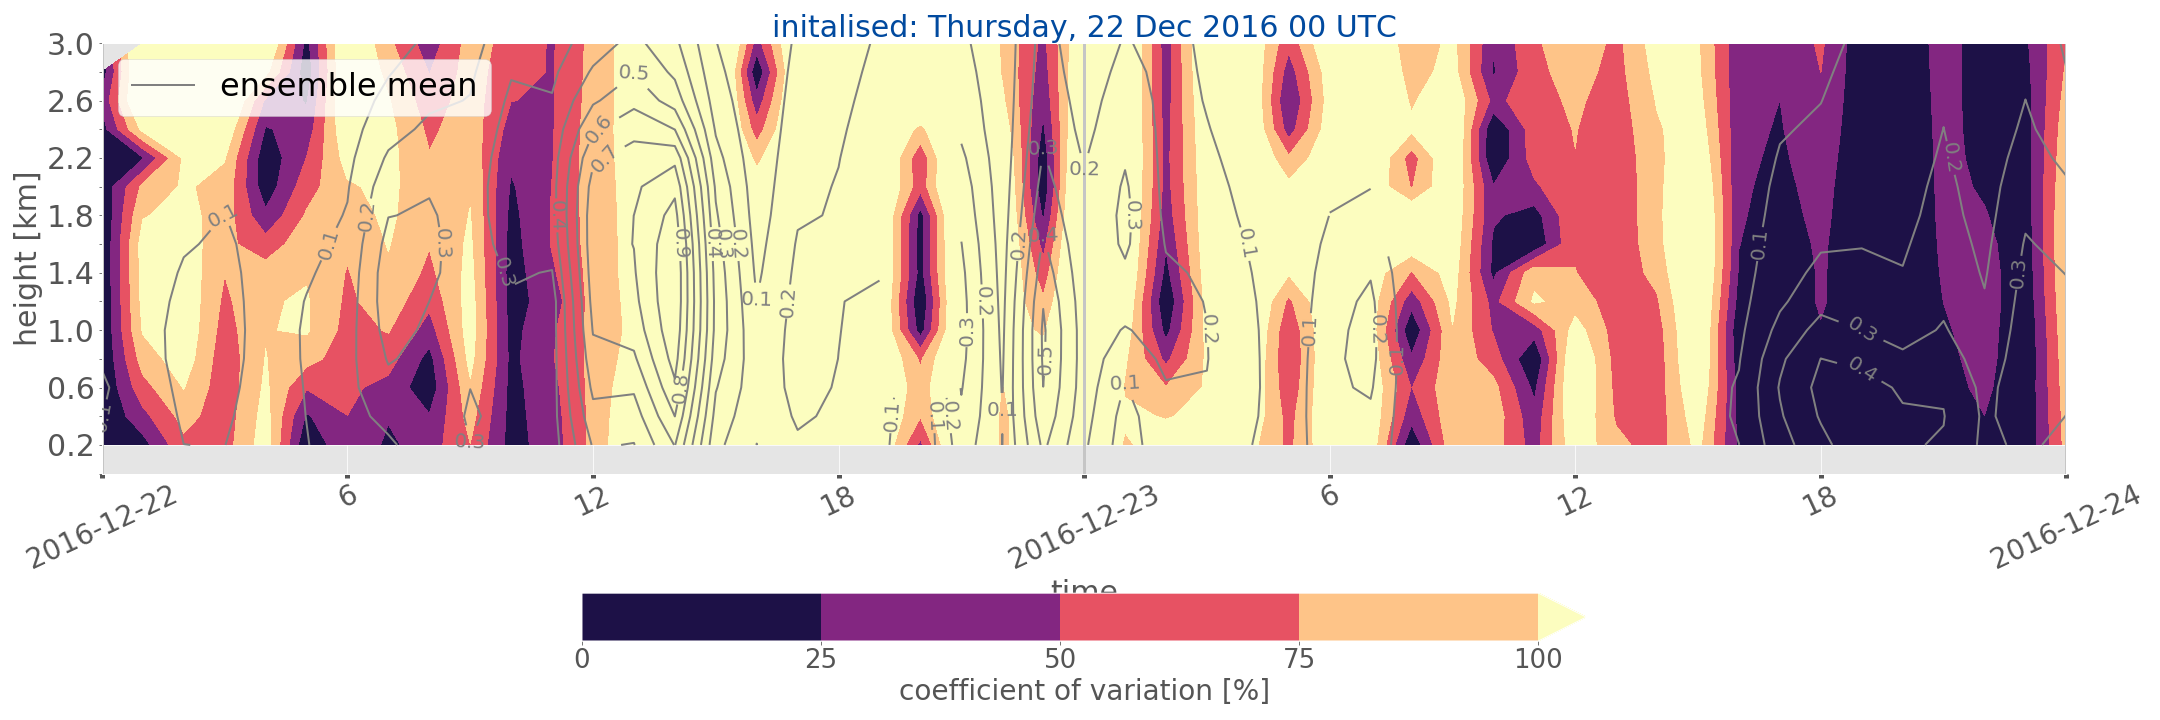
\includegraphics[trim={0.cm 5.3cm 0cm 0cm},clip,width=\textwidth]{./fig_variation/20161222}
			\caption{}\label{fig:ens_vari22}
		\end{subfigure}
    % 23/12
% 		\begin{subfigure}[t]{\textwidth}		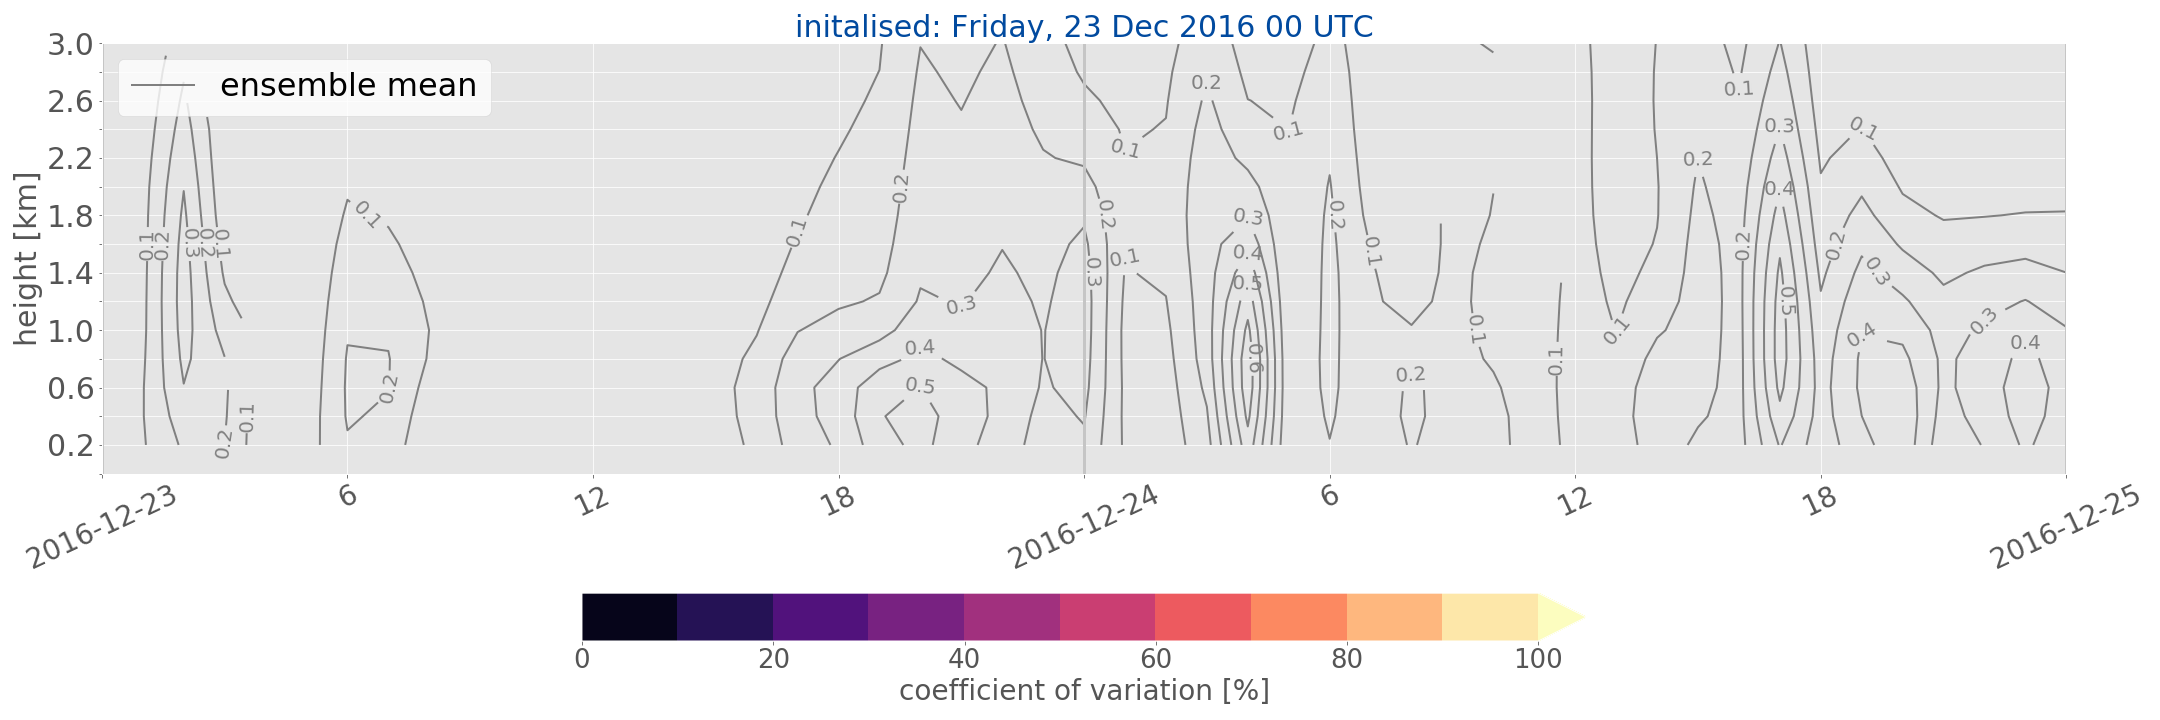
\includegraphics[trim={0.cm 0cm 0cm 0cm},clip,width=\textwidth]{./fig_variation/20161223}
% 			\caption{}\label{fig:ens_vari23}
% 		\end{subfigure}
    % 24/12
		\begin{subfigure}[t]{\textwidth}		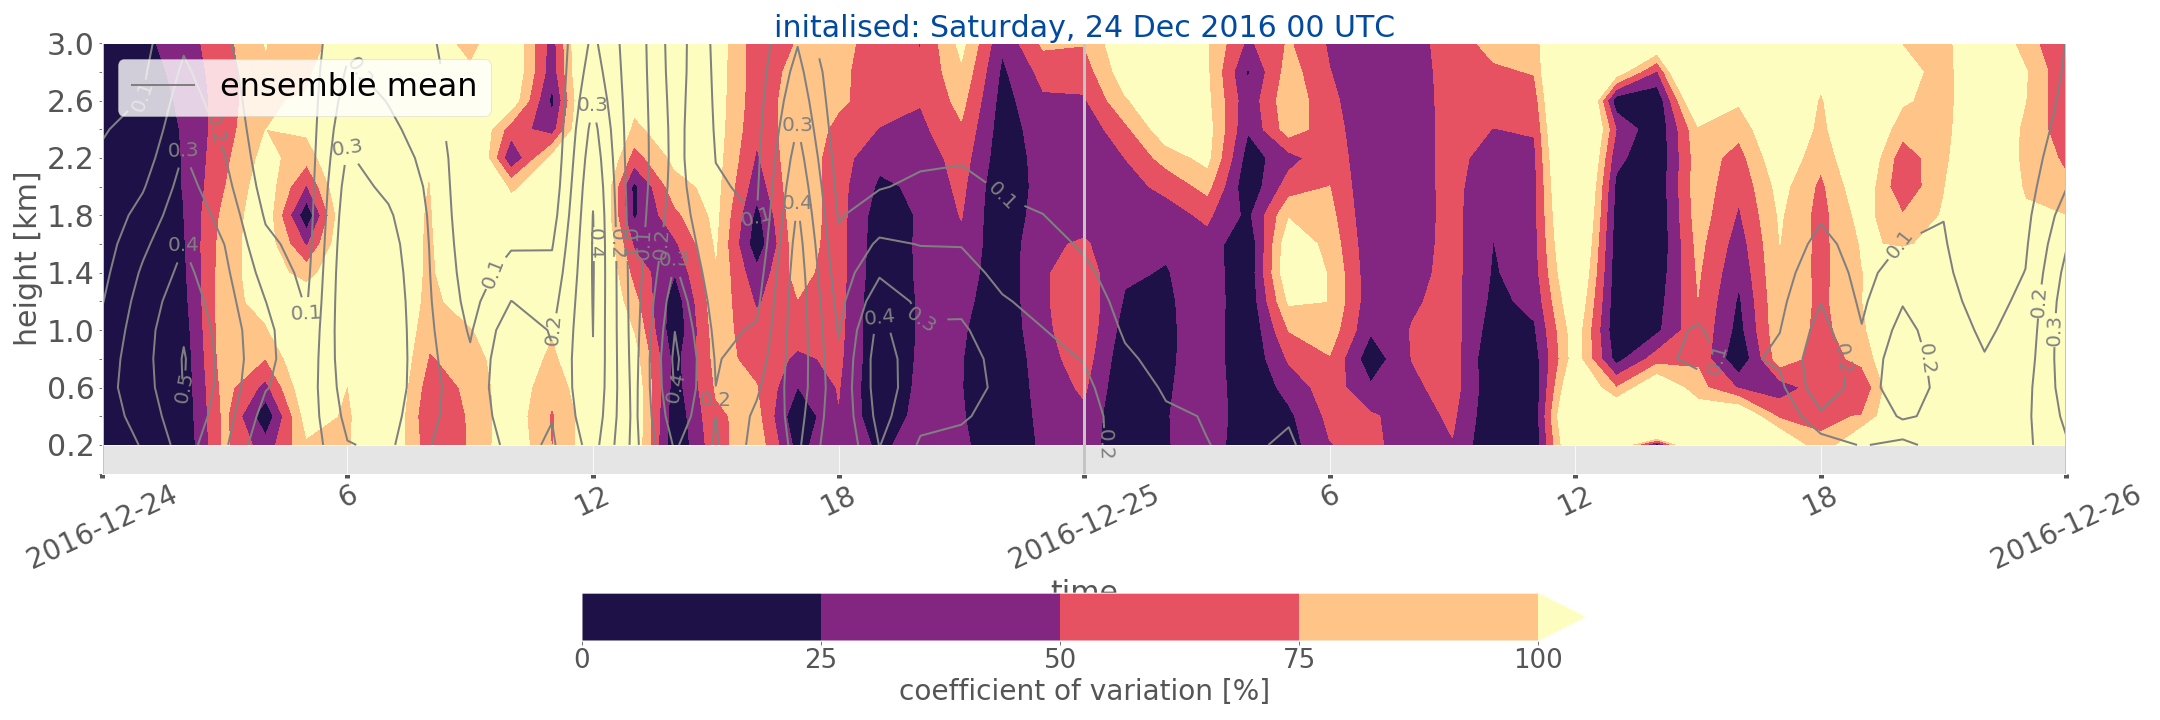
\includegraphics[trim={0.cm 5.3cm 0cm 0cm},clip,width=\textwidth]{./fig_variation/20161224}
			\caption{}\label{fig:ens_vari24}
		\end{subfigure}
        
     % colourbar
     	\begin{subfigure}[t]{\textwidth}		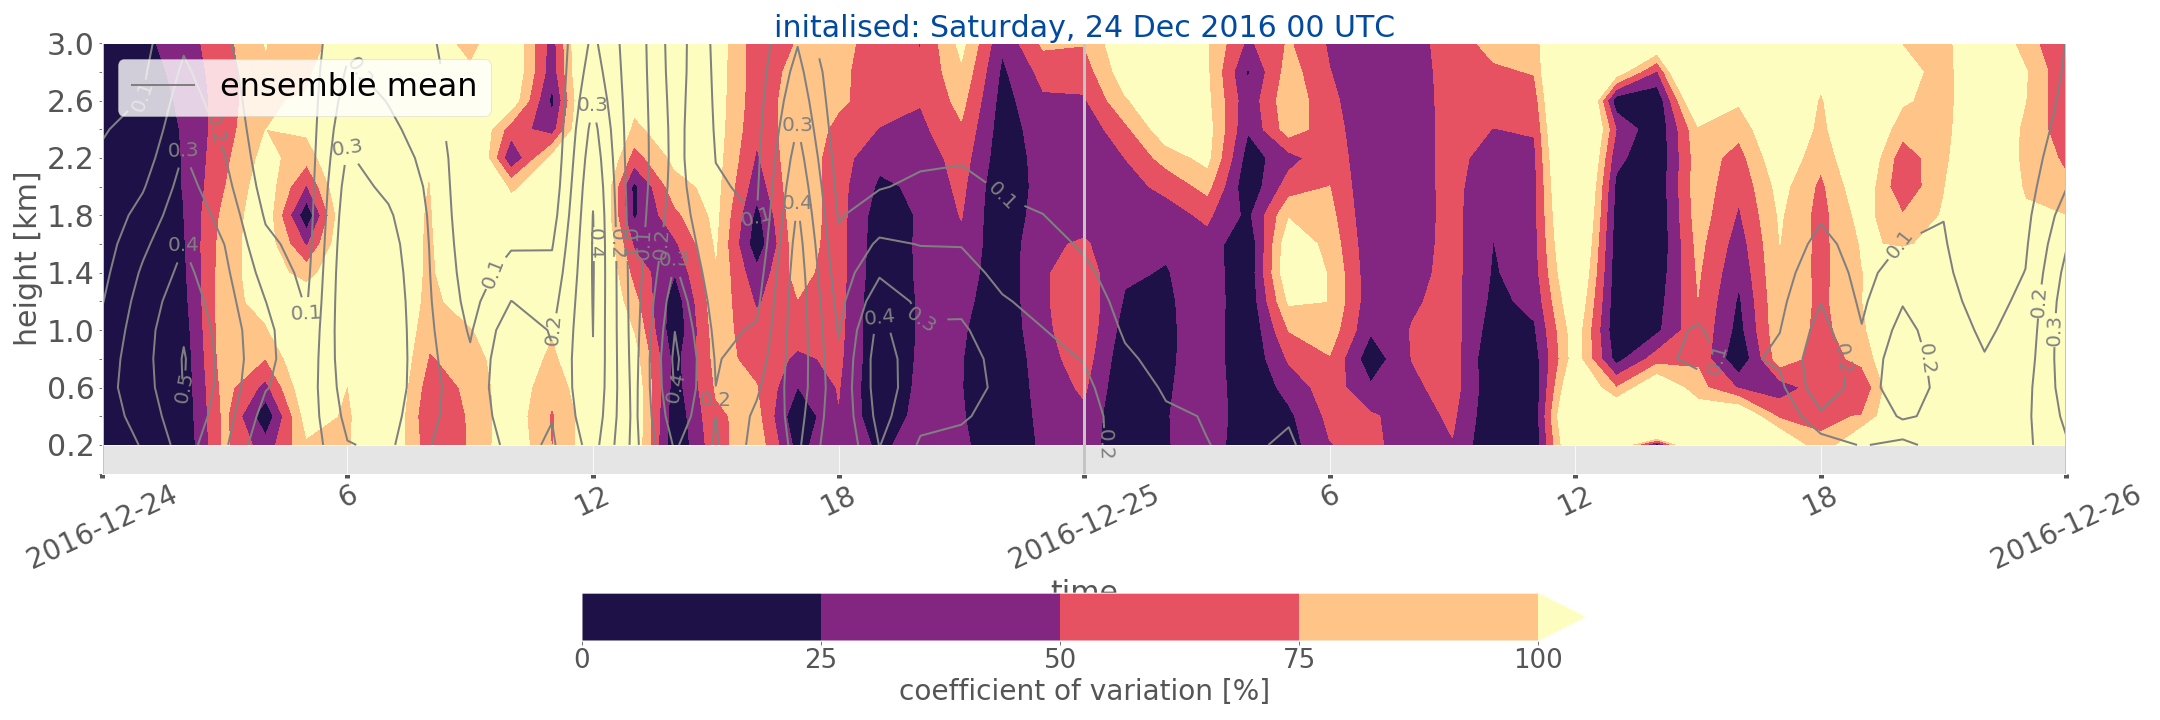
\includegraphics[trim={15.cm 0cm 15cm 21cm},clip,width=\textwidth]{./fig_variation/20161224}
		\end{subfigure}
\end{figure}
\begin{figure}[t]\ContinuedFloat
	\centering
    % 25/12
		\begin{subfigure}[t]{\textwidth}		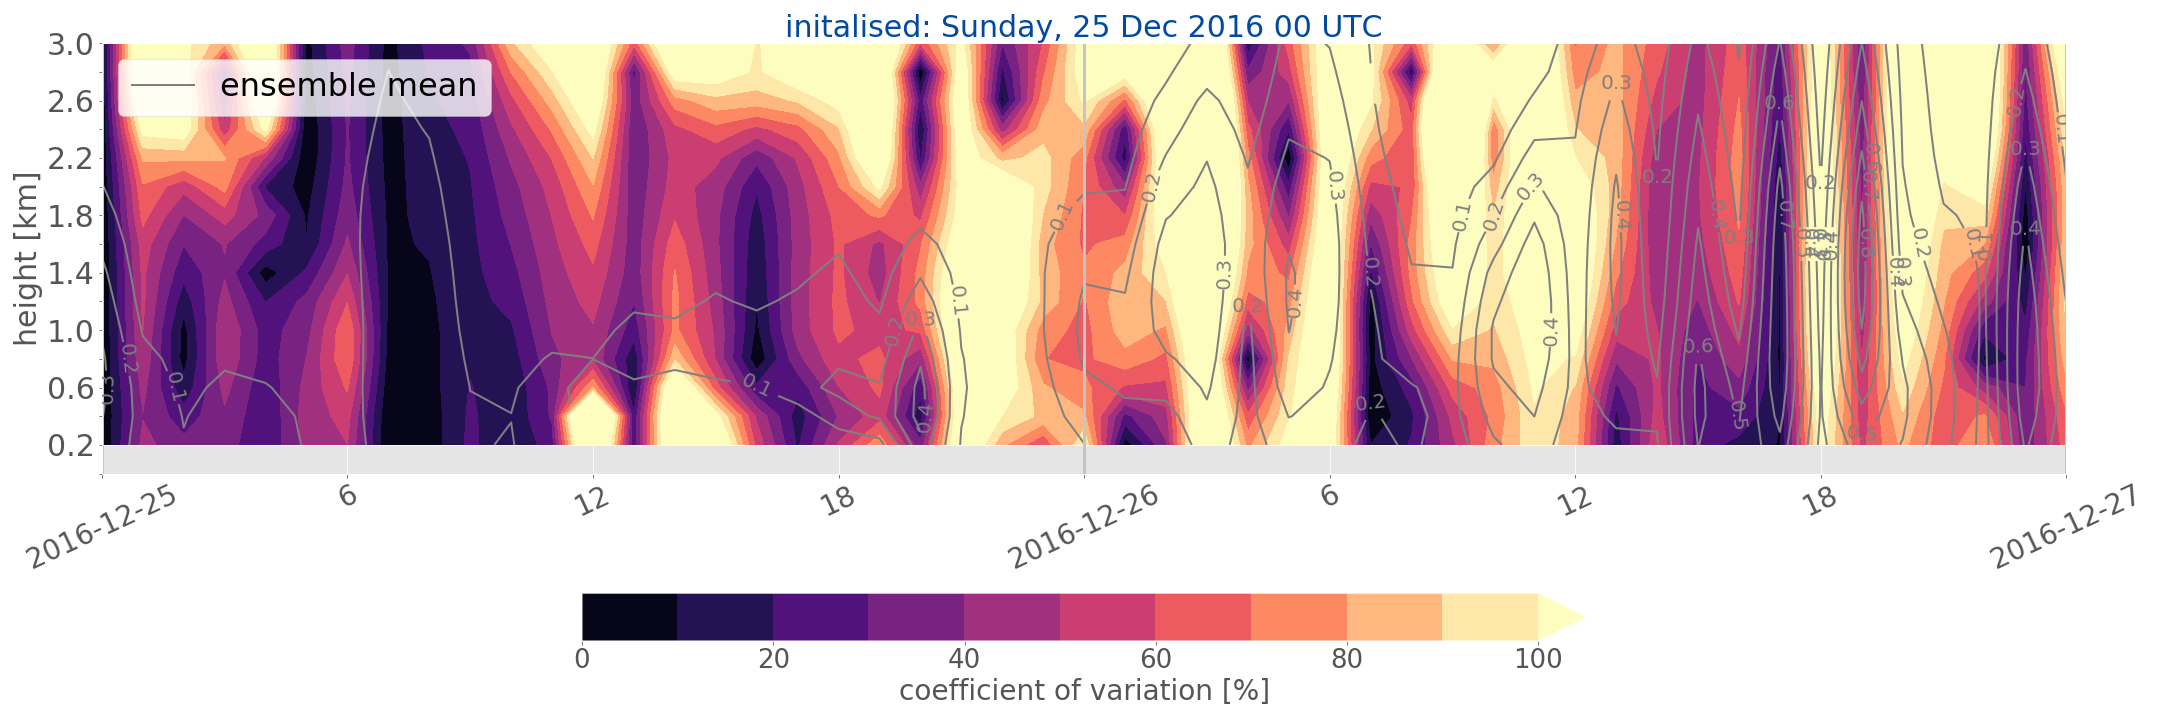
\includegraphics[trim={0.cm 5.3cm 0cm 0cm},clip,width=\textwidth]{./fig_variation/20161225}
			\caption{}\label{fig:ens_vari25}
		\end{subfigure}
    % 26/12
		\begin{subfigure}[t]{\textwidth}		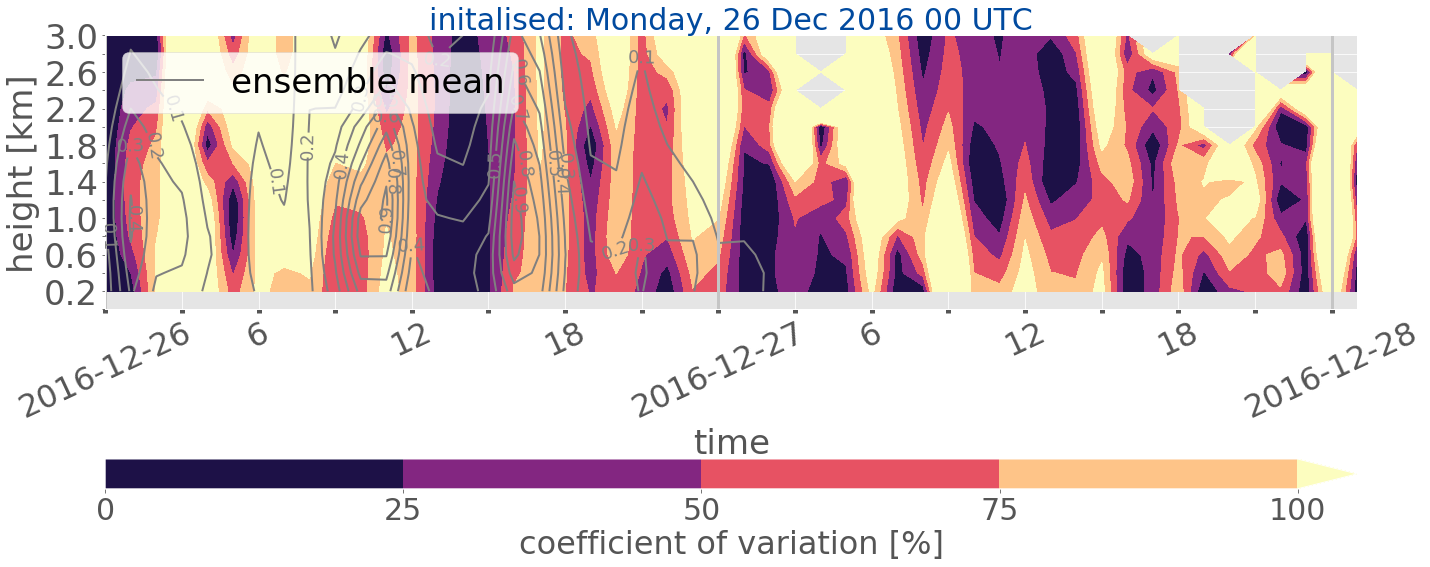
\includegraphics[trim={0.cm 5.3cm 0cm 0cm},clip,width=\textwidth]{./fig_variation/20161226}
			\caption{}\label{fig:ens_vari26}
		\end{subfigure}
%     % 27/12
% 		\begin{subfigure}[t]{\textwidth}		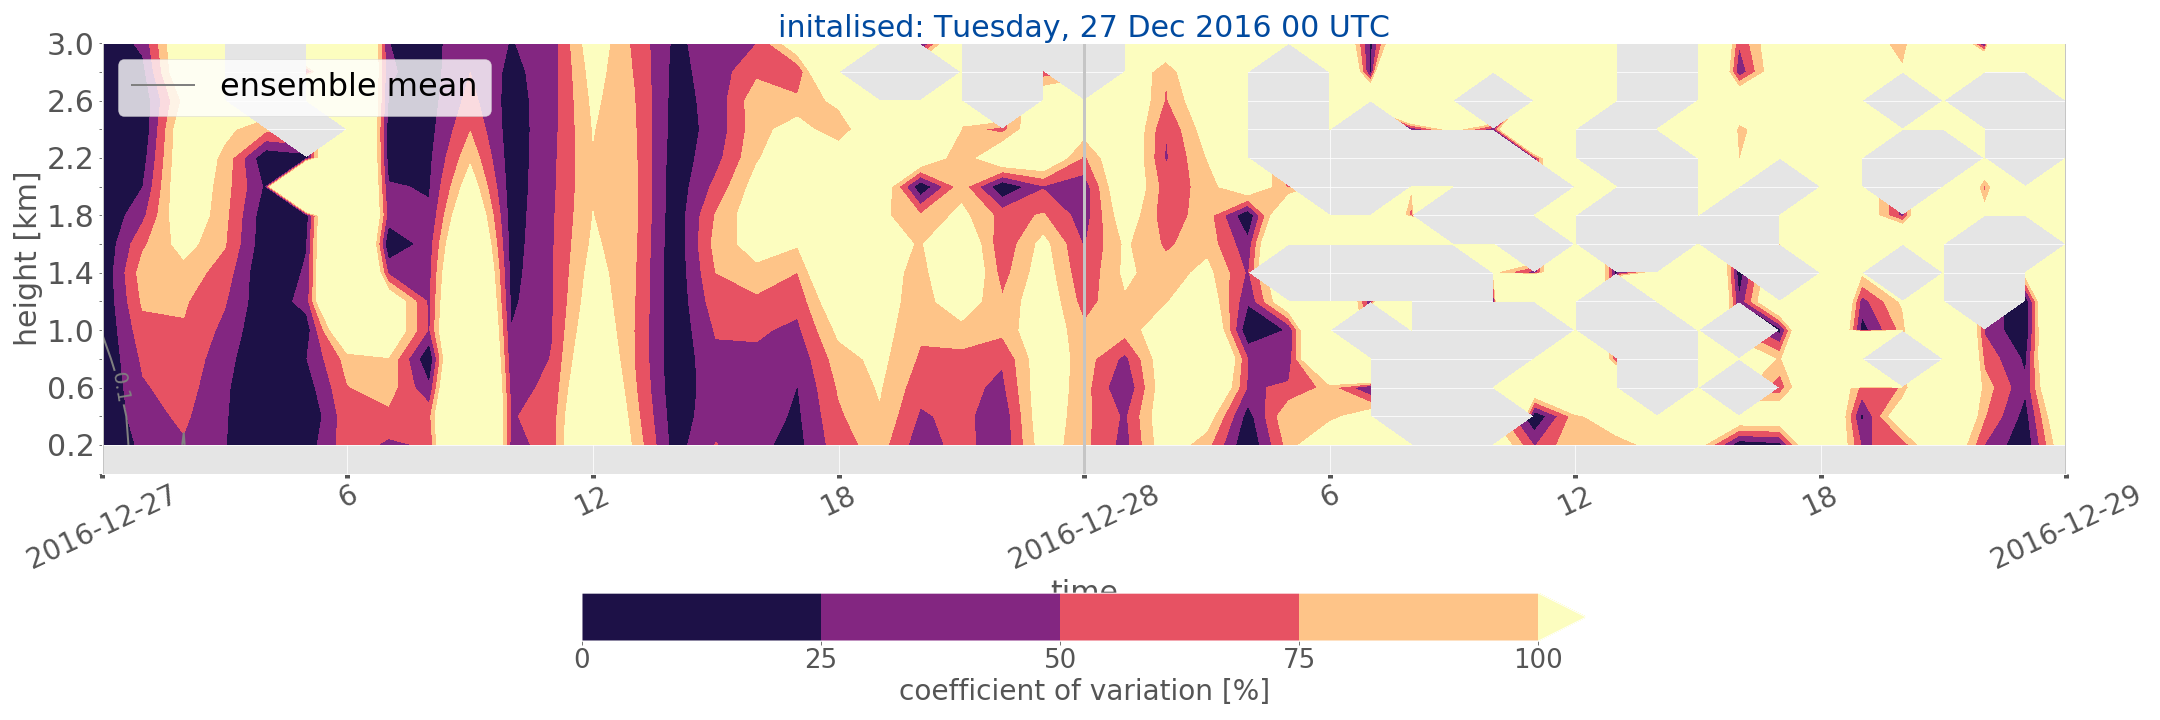
\includegraphics[trim={0.cm 5.3cm 0cm 0cm},clip,width=\textwidth]{./fig_variation/20161227}
% 			\caption{}\label{fig:ens_spread27}
% 		\end{subfigure}
        
    % colourbar
     	\begin{subfigure}[t]{\textwidth}		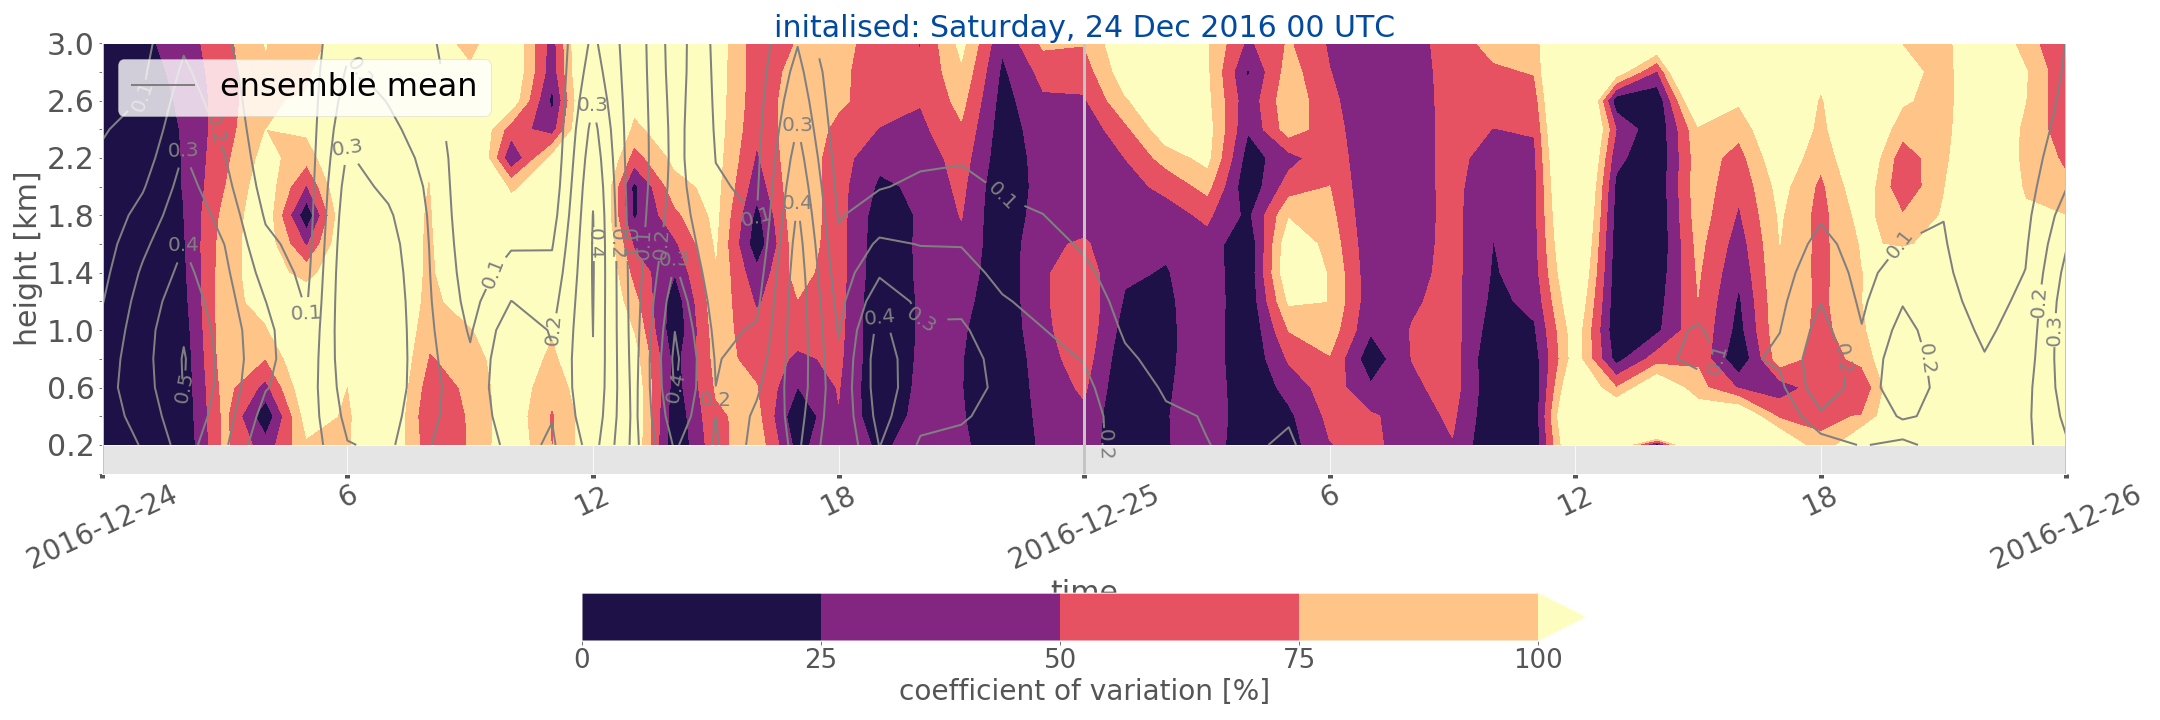
\includegraphics[trim={15.cm 0cm 15cm 21cm},clip,width=\textwidth]{./fig_variation/20161224}
		\end{subfigure}
        \caption{SWC variation of the ten ensemble members of MEPS. The lighter the colour according to the colourbar the higher the variation between the perturbed ensemble members. In grey the ensemble mean of all ten members.}\label{fig:ens_vari}
\end{figure}

